\subsection{ALIAS - existing implementation}
As shown in section \ref{section:alias}, ALIAS \citep{alias} is the pure Python implementation of abstract argumentation semantics solver. It is using a direct approach for solving the semantics by enumerating all possible sets from the given argumentation framework and verifying them individually for complete, preferred and stable extensions. Although this approach can guarantee to produce the correct output, given the verification process is correct, it is highly inefficient and resource intensive. 

ALIAS can also produce the labellings for complete, grounded, preferred, stable and semi-stable semantics, by iterating through the whole argumentation framework and label the arguments accordingly. Once the solution is created it breaks out of the loop and outputs the labellings. Hence, although ALIAS has a lot of functionality in terms of computing abstract argumentation semantics, the implementation method used for the solver makes it inefficient and difficult to work on the larger frameworks. 

The benefit of ALIAS is its ability to read and parse argumentation frameworks from multiple input formats. In the existing implementation, Apart from standard input of tgf (Trivial Graph Format) and apx (Ability Photopaint Studio Image) files, ALIAS also support input from JSON, DOT graph, networkx and databases SQLLite, mySql and Neo4j. Furthermore, it is possible ot output the argumentation framework into those formats as well.

Although current implementation of ALIAS don't have any mandatory dependencies, additional dependencies are required to allow for additional functionality:
\begin{itemize}
	\item Input/Output
	\begin{itemize}
		\item pyparsing - module for file input and output
		\item networkx - used for conversion to and from NetworkX graphs 
	\end{itemize}
	\item Databases
	\begin{itemize}
		\item sqlalchemy - required for interaction with SQL based databases
		\item py2neo - used with neo4j graph databases
	\end{itemize}
	\item Testing
	\begin{itemize}
		\item nose - Nose Testing Framework
	\end{itemize}
\end{itemize}

Those dependencies can be easily installed through setup script if required. 

\subsubsection{ALIAS Structure}
Currently ALIAS is made of 3 modules: 

\begin{itemize}
	\item classes - consist of classes representing argumentation framework, arguments and labelling
	\item inout - module responsible for input and output from and to different file formats
	\item semantics - collection of static methods used for computing extensions and labellings of given argumentation framework.
\end{itemize}

This structure and the relations between them can be seen in figure \ref{fig:aliasUml1}. Inout and semantics modules requires framework class from classes module. Otherwise, there are no connections between each individual package.

\begin{figure}[h]
	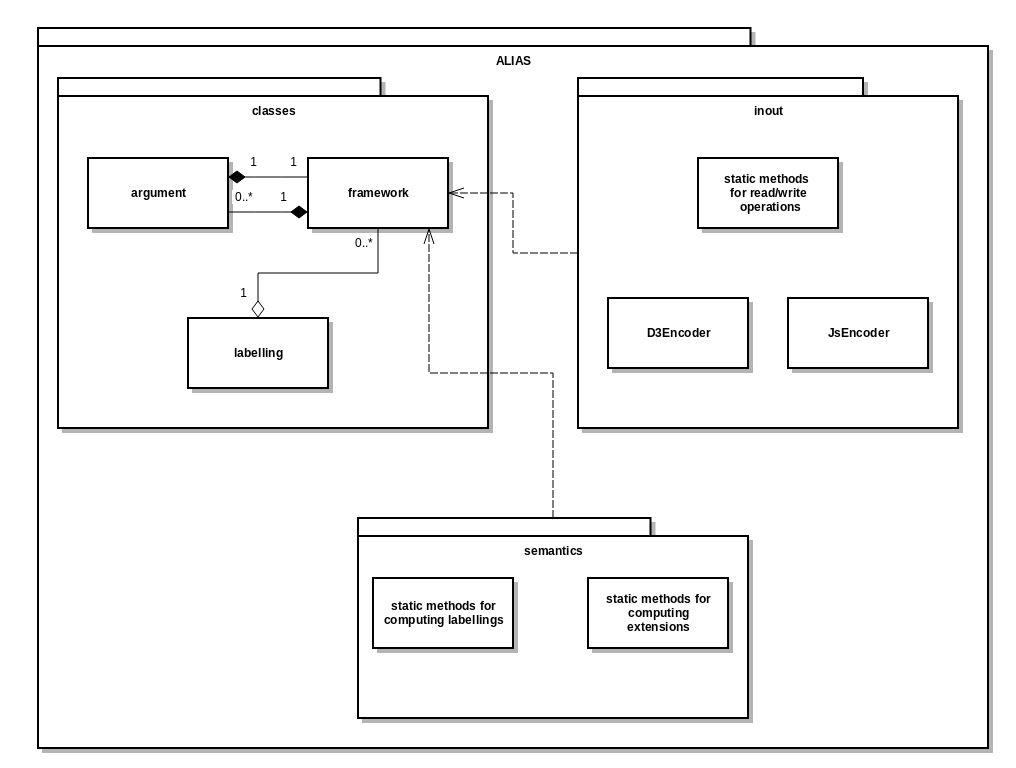
\includegraphics[width=\textwidth]{alias_current_uml}
	\caption{ALIAS UML diagram}
	\label{fig:aliasUml1}
\end{figure}



\begin{landscape}
	\begin{figure}
		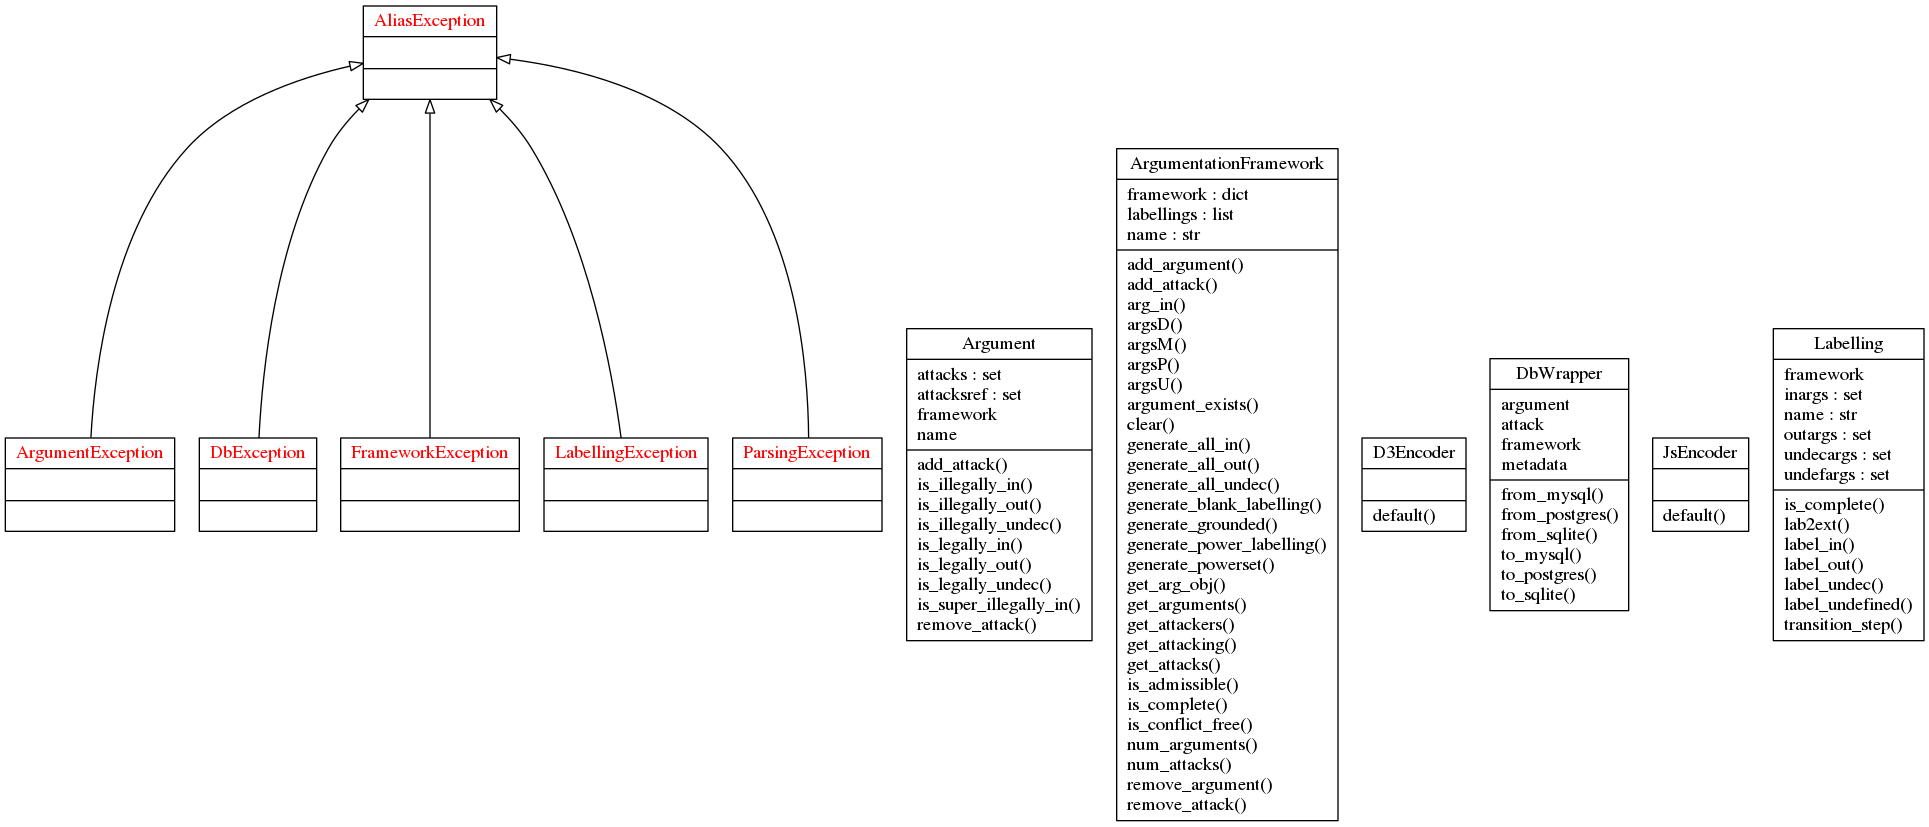
\includegraphics[width=21cm]{alias1}
		\caption{ALIAS Class breakdown}
		\label{fig:aliasClassBreakdown}
	\end{figure}
\end{landscape}

\subsubsection{Performance}
As mentioned above, current implementation of ALIAS generates a power set from all arguments within the argumentation framework and checks each of them to create the solution. As can be seen in figure \ref{fig:aliasPerResults}, the time required to compute Stable extensions grows exponentially with the size of the argumentation framework. 

\begin{figure}[h]
	\centering
	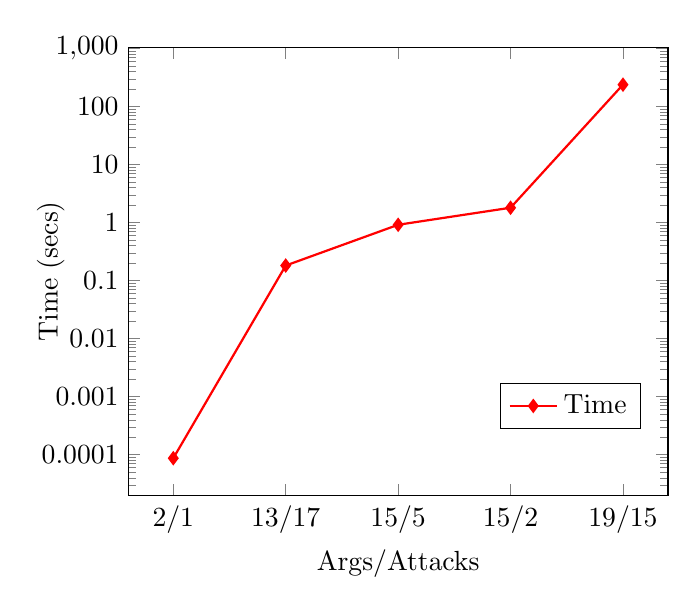
\begin{tikzpicture}
		\begin{semilogyaxis}
		[
		log ticks with fixed point,
		xlabel=Args/Attacks,
		ylabel=Time (secs),
		symbolic x coords={2/1, 13/17, 15/5, 15/2, 19/15},
		xtick=data,
	    x label style={at={(axis description cs:0.5,-0.1)},anchor=north},
	    y label style={at={(axis description cs:-0.1,.5)},anchor=south},
		legend style={at={(0.95,0.2)},anchor=east}
		]

	\addplot[mark=diamond*,thick,red] coordinates {
		(2/1,0.000087)
		(13/17,0.1819)
		(15/5, 0.9173)
		(15/2, 1.8042)
		(19/15, 238.425)
	};
	\legend{Time}
	\end{semilogyaxis}
	\end{tikzpicture}
	
	\caption{ALIAS Performance Results for Stable Extensions}
	\label{fig:aliasPerResults}
	
\end{figure}

Furthermore, the approach of creating a power set from all arguments within the framework is memory intensive. Figure \ref{fig:bytesPowerSet} shows how much memory in bytes is required to store a power set based on the number of elements. As it can be seen the memory usage is exponentially growing with every additional element in the list. Thus, with this approach, the available memory can quickly be used for storing the power set of all arguments, making the machine ALIAS is run on, unusable.

\begin{figure}[h]
	\centering
	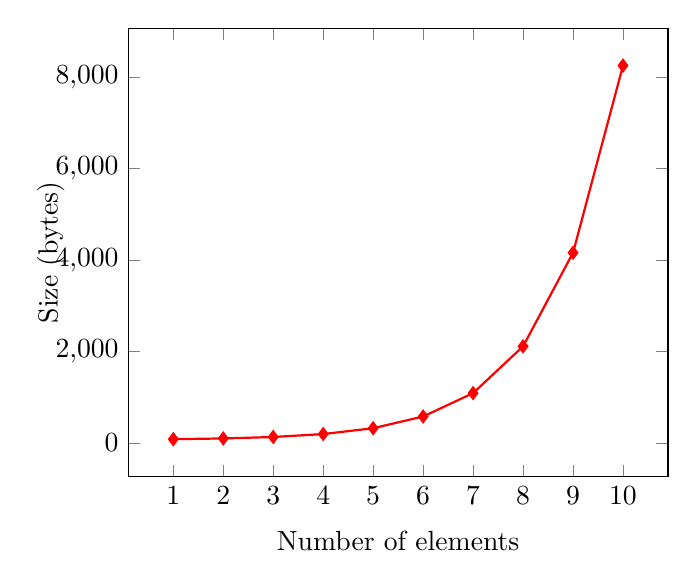
\begin{tikzpicture}
	\begin{axis}
	[
	log ticks with fixed point,
	xlabel=Number of elements,
	ylabel=Size (bytes),
	symbolic x coords={1,2,3,4,5,6,7,8,9,10},
	xtick=data,
	x label style={at={(axis description cs:0.5,-0.1)},anchor=north},
	y label style={at={(axis description cs:-0.1,.5)},anchor=south},
	legend style={at={(0.95,0.2)},anchor=east}
	]
	
	\addplot[mark=diamond*,thick,red] coordinates {
		(1,80)
		(2,96)
		(3,128)
		(4,192)
		(5,320)
		(6,576)
		(7,1088)
		(8,2112)
		(9,4160)
		(10,8256)
	};
	\end{axis}
	\end{tikzpicture}
	
	\caption{Size of Power Set in bytes}
	\label{fig:bytesPowerSet}
	
\end{figure}
